\section{Gegen\"uberstellung aller Feldbilder der Kurzschlussanordnungen aus der CST Simulation}
\label{sec:allfieldplots}
\begin{figure}[htb]
	\centering
	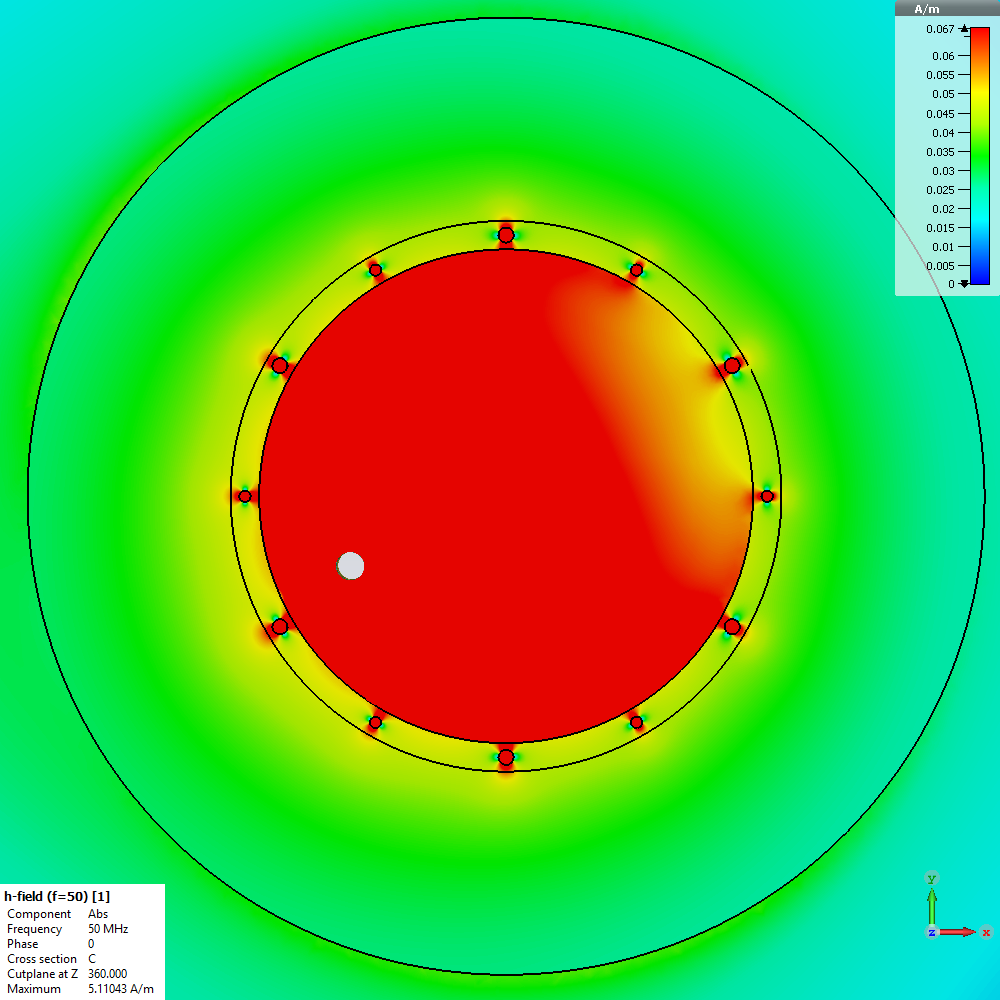
\includegraphics[width=0.5\textwidth]{Feldbilder/0KS}
	\caption{Feldbild des Ringkerns ohne Kurzschl\"usse aus der CST Simulation.}
	\label{fig:field0ks}
\end{figure}

\begin{figure}[htb]
	\centering
	\subfloat[1 Kurzschluss der Breite $\SI{20}{\milli\meter}$ und der h\"ohe $\SI{160}{\milli\meter}$.]{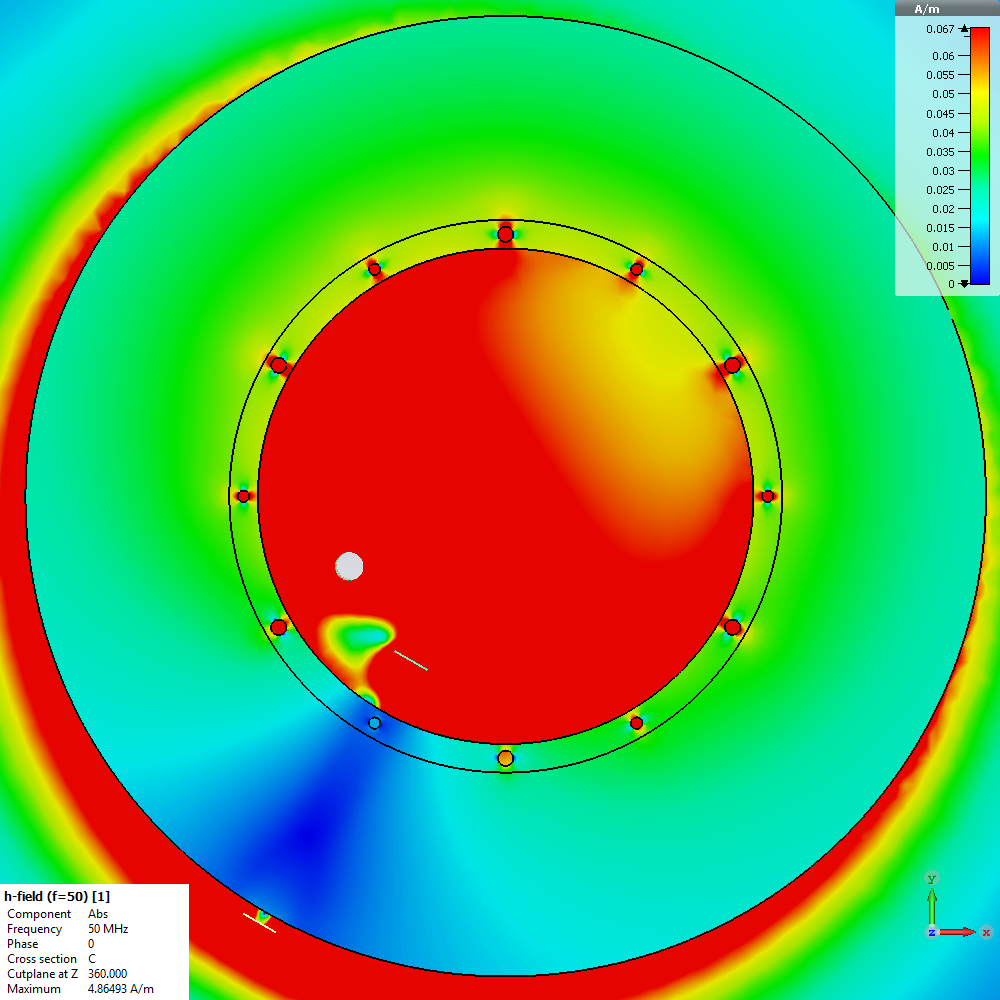
\includegraphics[width=0.33\textwidth]{Feldbilder/1KSb20}}
	\subfloat[1 Kurzschluss der Breite $\SI{30}{\milli\meter}$ und der h\"ohe $\SI{160}{\milli\meter}$.]{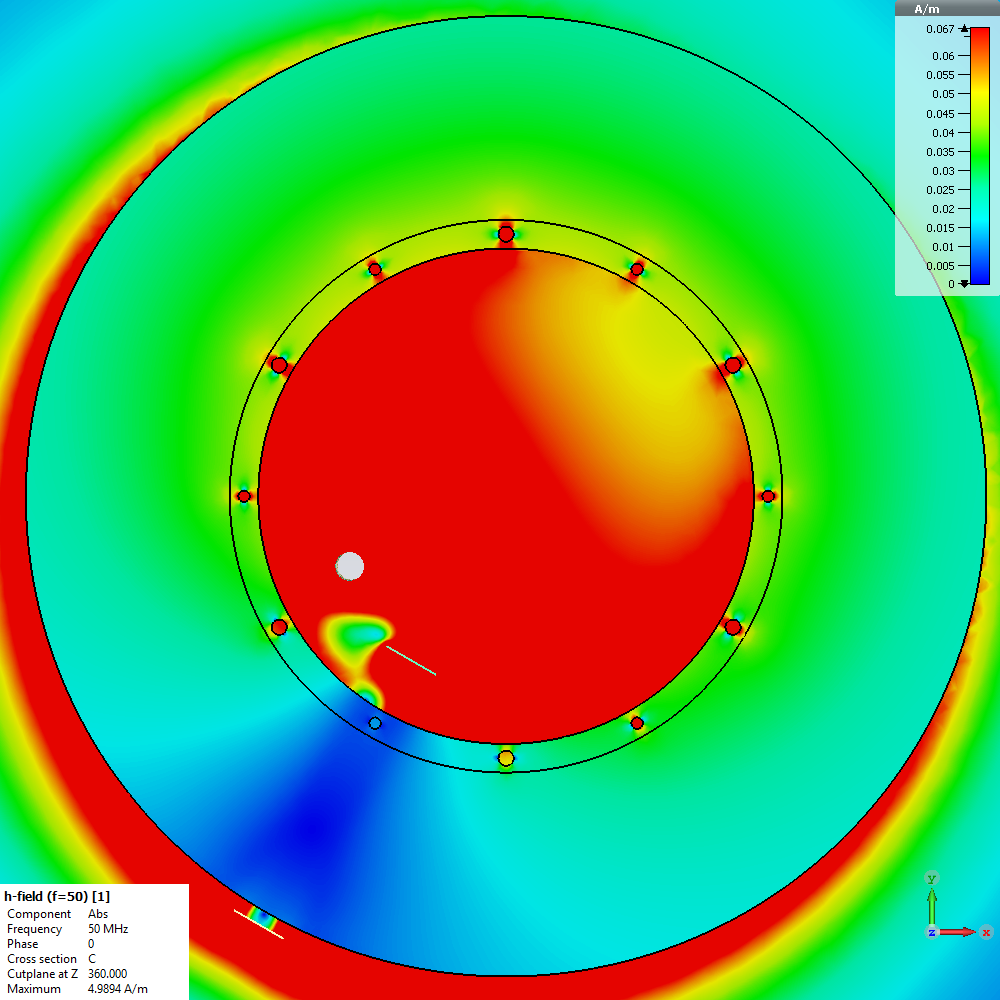
\includegraphics[width=0.33\textwidth]{Feldbilder/1KS}}
	\subfloat[1 Kurzschluss der Breite $\SI{50}{\milli\meter}$ und der h\"ohe $\SI{160}{\milli\meter}$.]{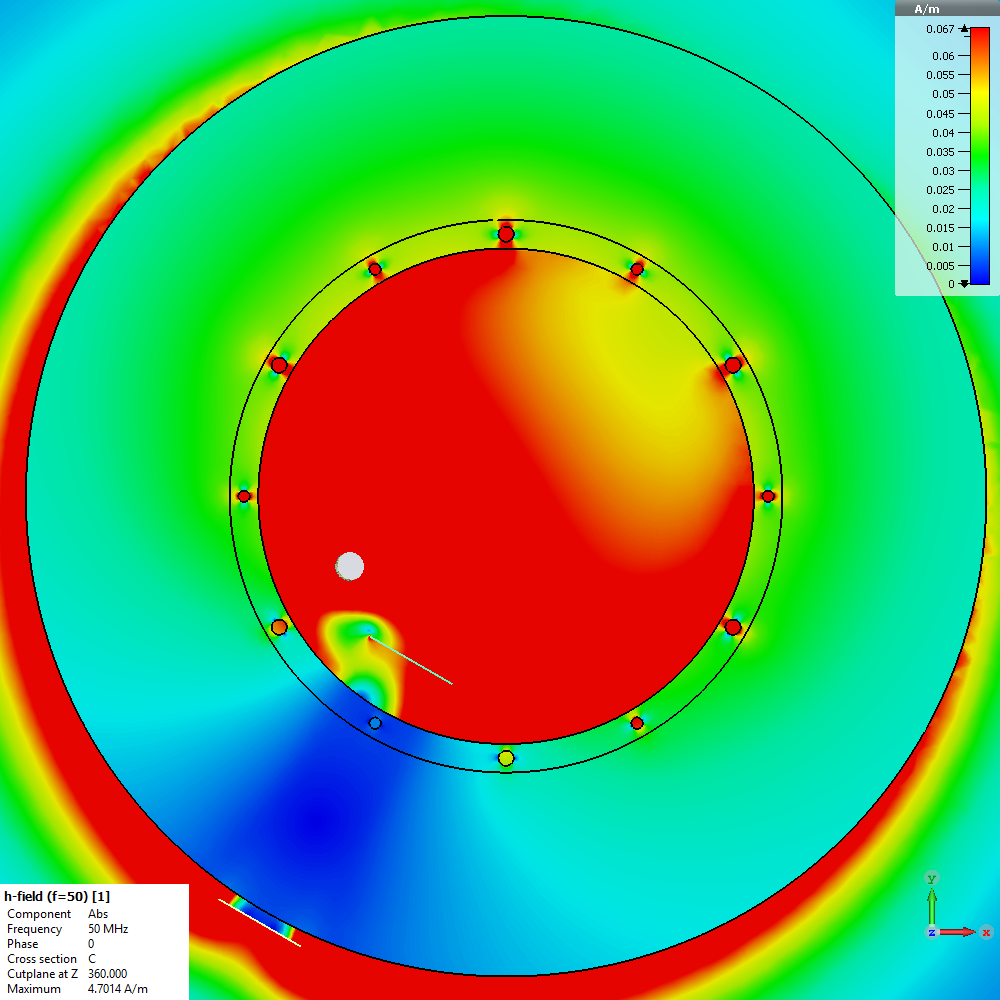
\includegraphics[width=0.33\textwidth]{Feldbilder/1KSb50}}
	\caption{Gegen\"uberstellung der Feldbilder des Ringkerns mit jeweils einem Kurzschluss verschiedener Breiten aus der CST Simulation.}
	\label{fig:field1ks}
\end{figure}

\begin{figure}[htb]
	\centering
	\subfloat[2 Kurzschl\"usse der Breite $\SI{20}{\milli\meter}$ und der h\"ohe $\SI{160}{\milli\meter}$.]{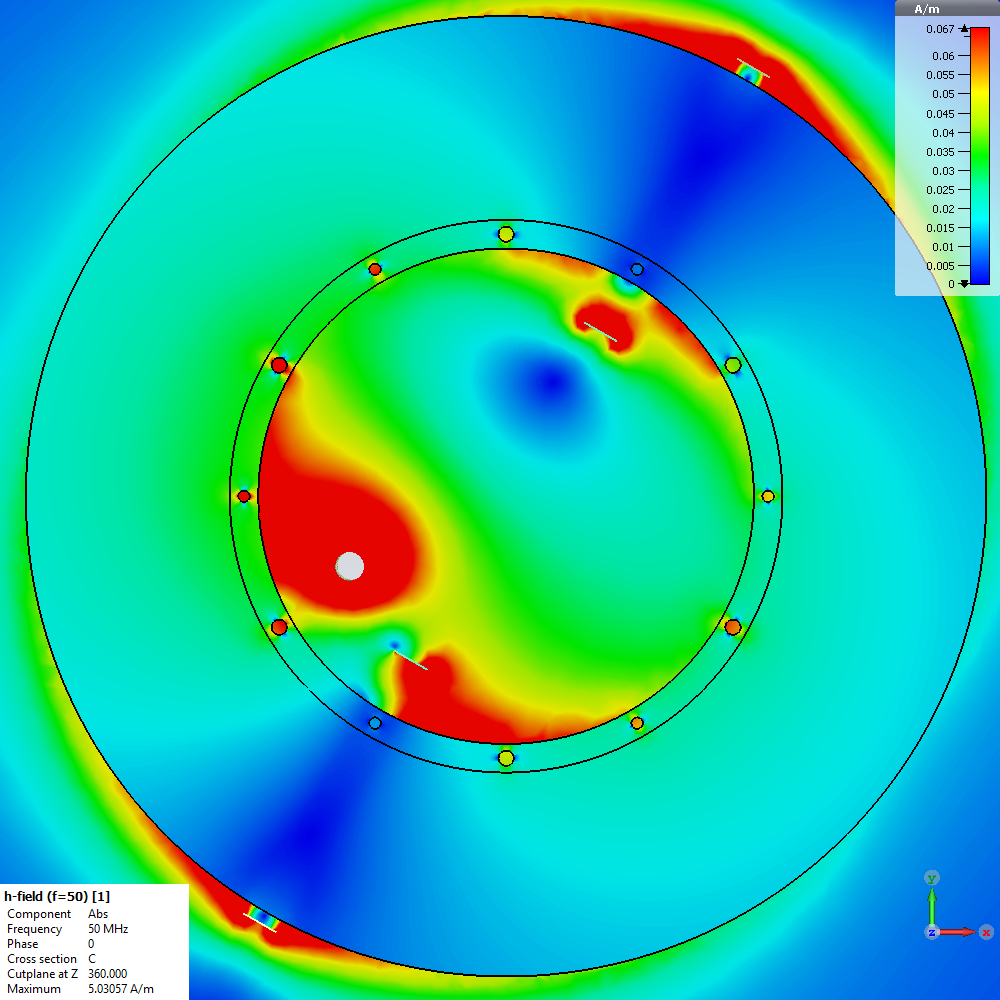
\includegraphics[width=0.33\textwidth]{Feldbilder/2KSb20}}
	\subfloat[2 Kurzschl\"usse der Breite $\SI{30}{\milli\meter}$ und der h\"ohe $\SI{160}{\milli\meter}$.]{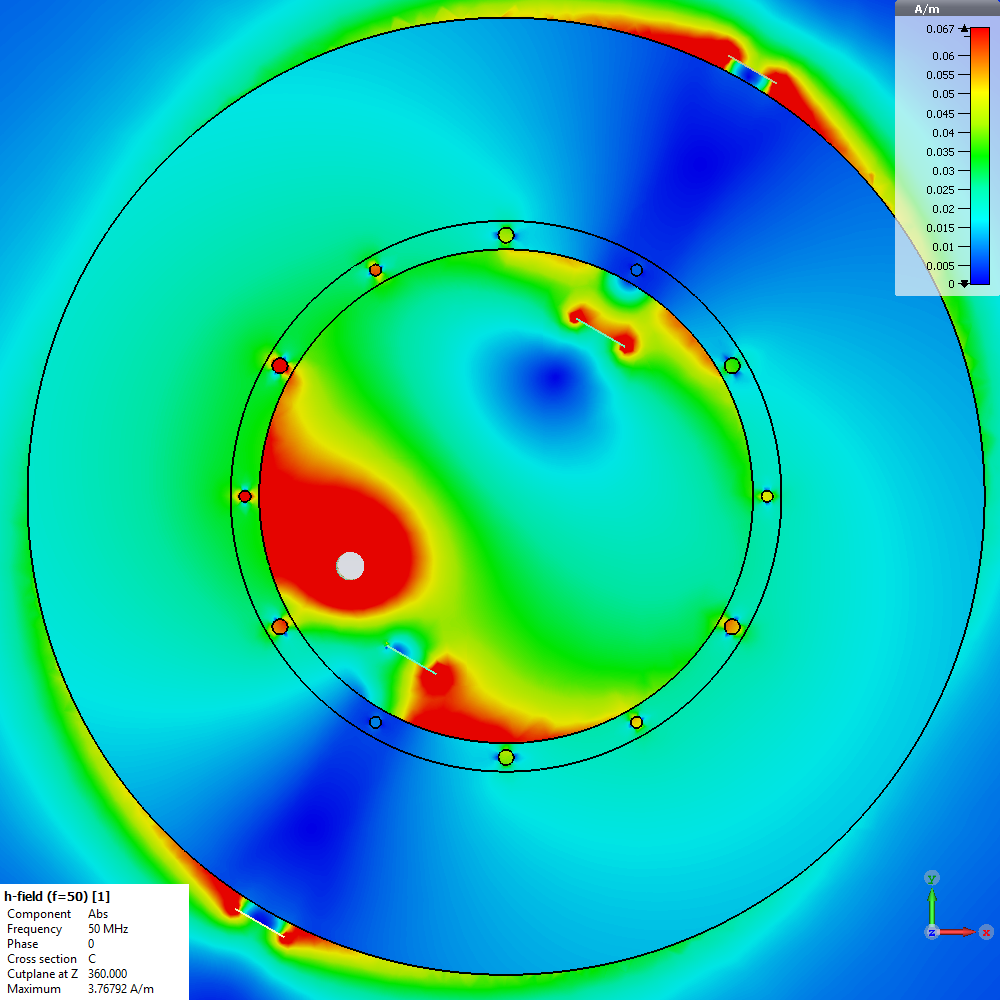
\includegraphics[width=0.33\textwidth]{Feldbilder/2KS}}
	\subfloat[2 Kurzschl\"usse der Breite $\SI{50}{\milli\meter}$ und der h\"ohe $\SI{160}{\milli\meter}$.]{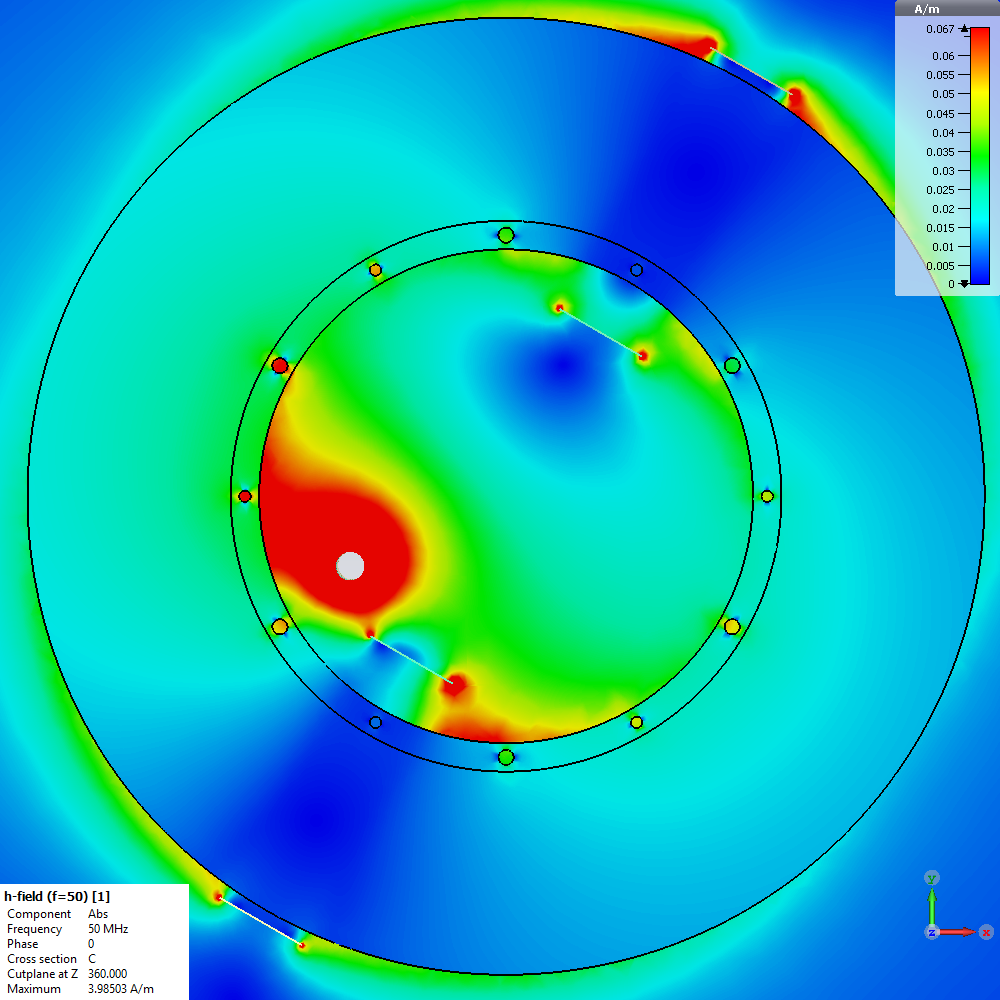
\includegraphics[width=0.33\textwidth]{Feldbilder/2KSb50}}
	\caption{Gegen\"uberstellung der Feldbilder des Ringkerns mit jeweils zwei Kurzschl\"ussen verschiedener Breiten aus der CST Simulation.}
	\label{fig:field2ks}
\end{figure}

\begin{figure}[htb]
	\centering
	\subfloat[3 Kurzschluss der Breite $\SI{30}{\milli\meter}$ und der h\"ohe $\SI{160}{\milli\meter}$.]{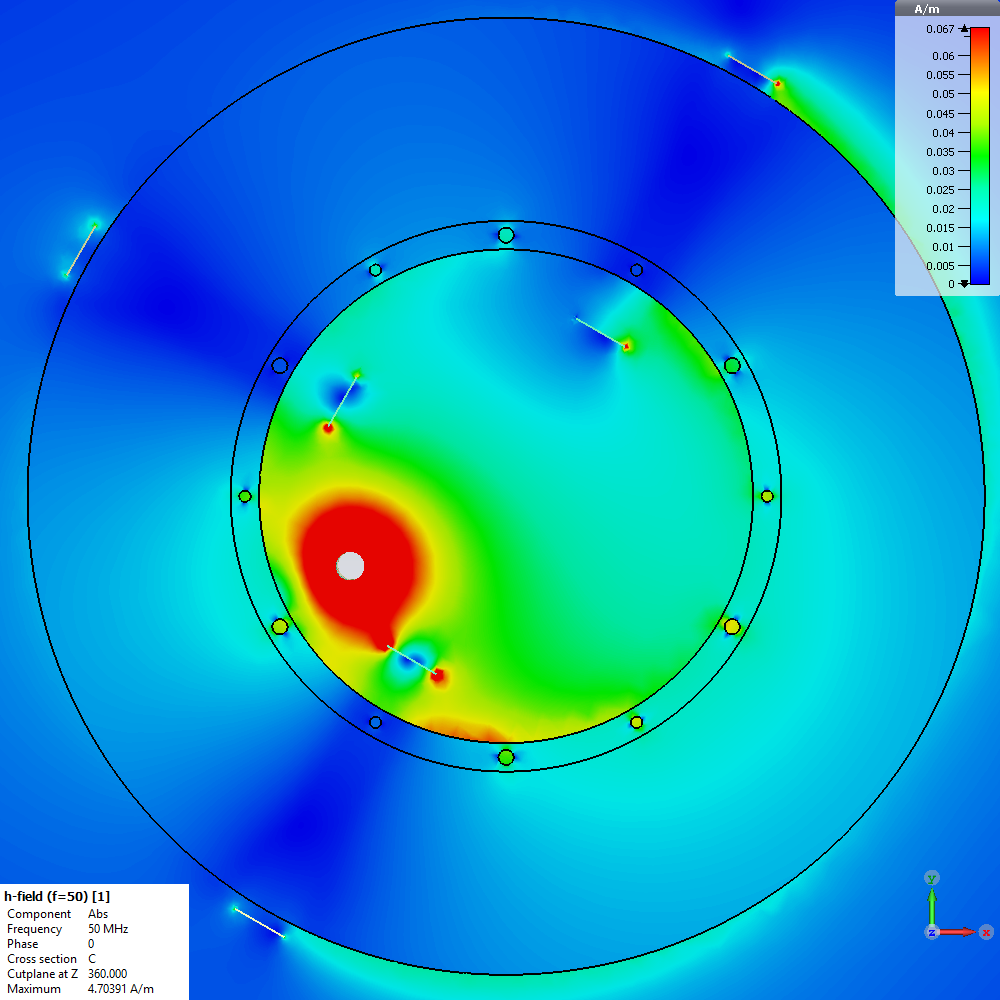
\includegraphics[width=0.33\textwidth]{Feldbilder/3KS}}
	\subfloat[4 Kurzschluss der Breite $\SI{30}{\milli\meter}$ und der h\"ohe $\SI{160}{\milli\meter}$.]{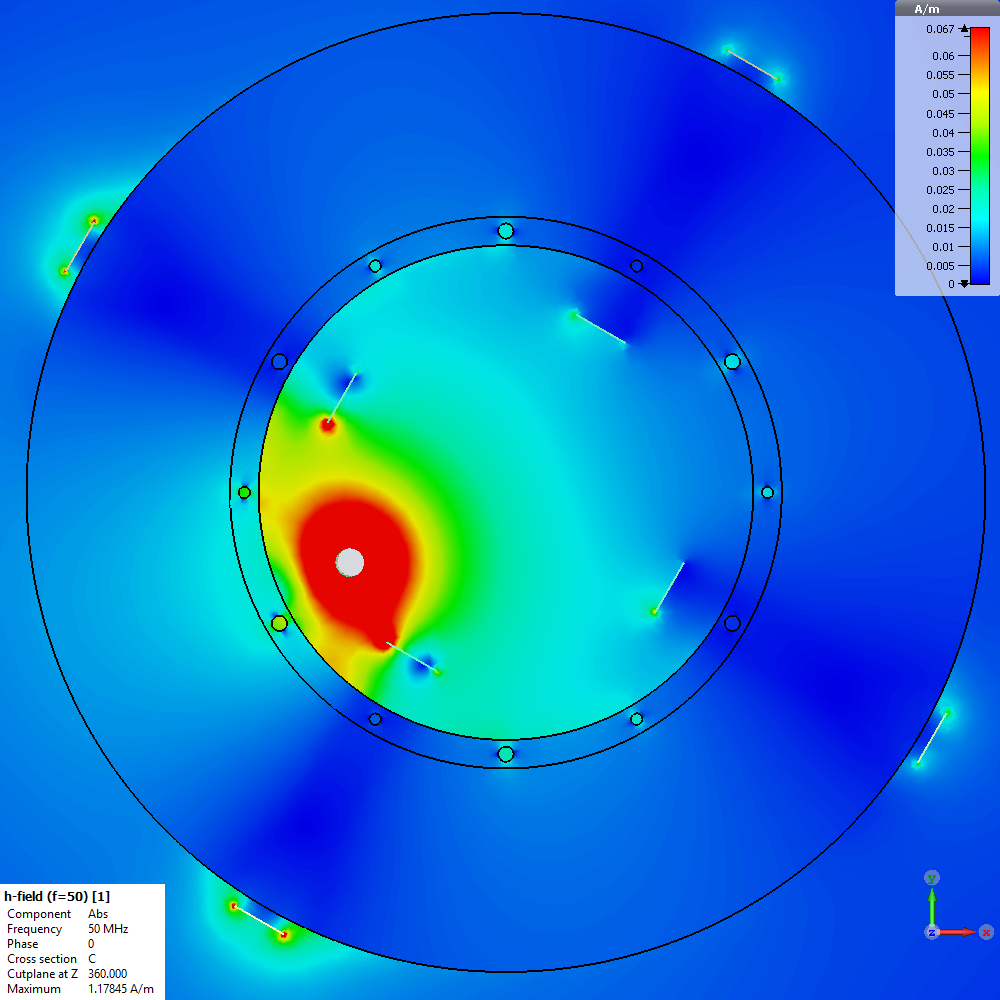
\includegraphics[width=0.33\textwidth]{Feldbilder/4KS}}
	\caption{Gegen\"uberstellung der Feldbilder des Ringkerns mit drei und vier Kurzschl\"ussen aus der CST Simulation.}
	\label{fig:field34ks}
\end{figure}

\begin{figure}[htb]
	\centering
	\subfloat[5 Kurzschluss der Breite $\SI{30}{\milli\meter}$ und der h\"ohe $\SI{160}{\milli\meter}$.]{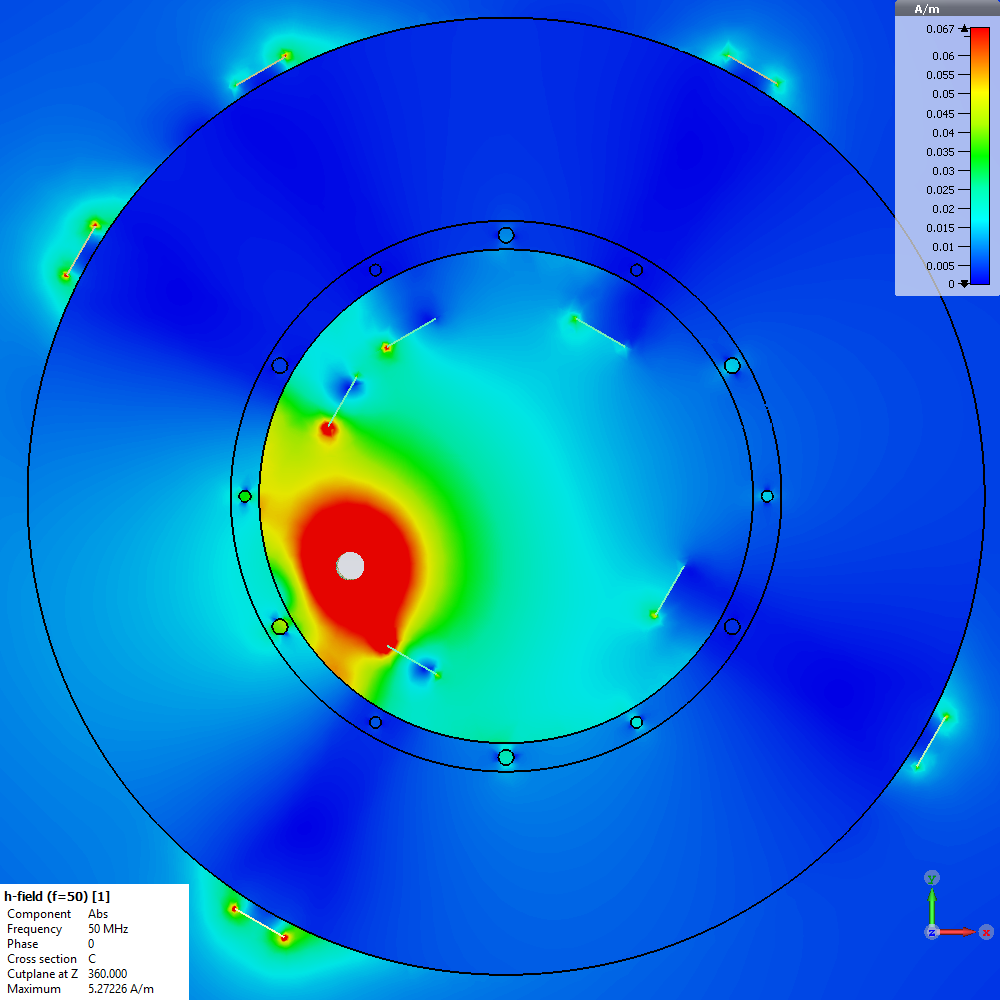
\includegraphics[width=0.33\textwidth]{Feldbilder/5KS}}
	\subfloat[6 Kurzschluss der Breite $\SI{30}{\milli\meter}$ und der h\"ohe $\SI{160}{\milli\meter}$.]{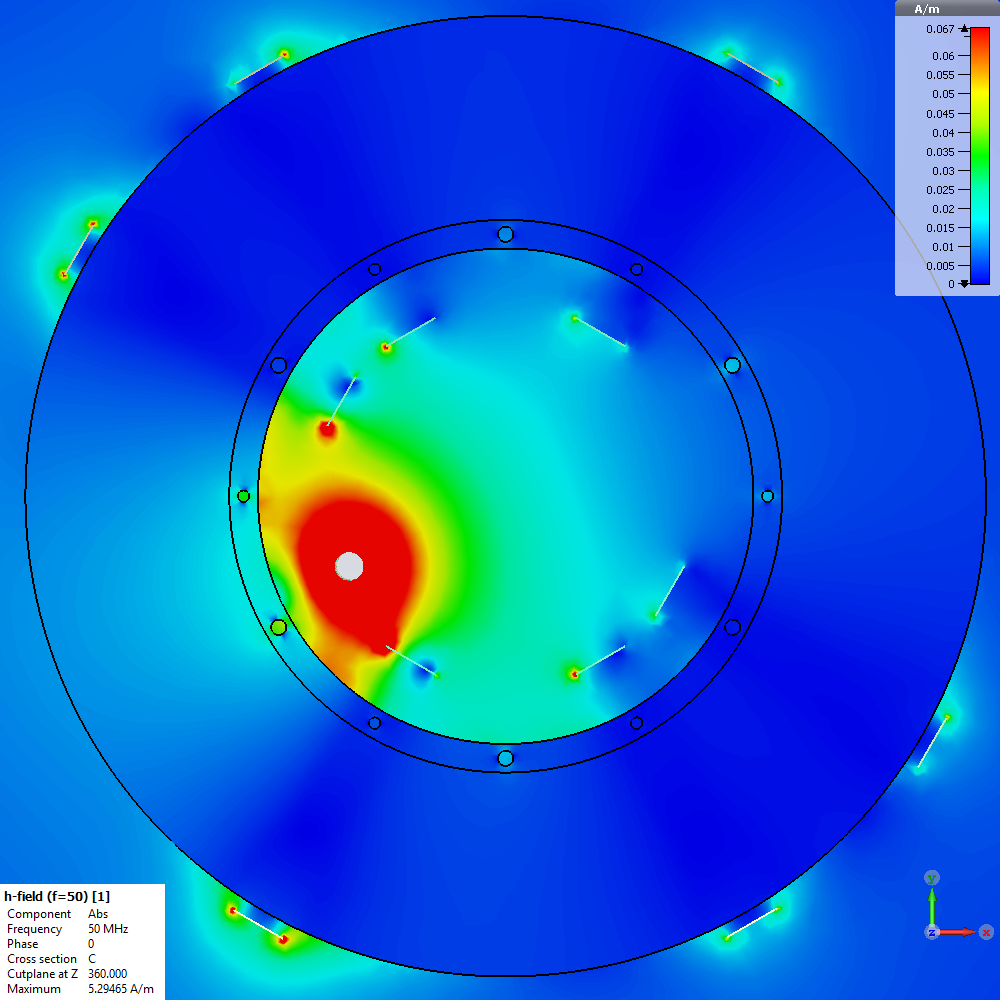
\includegraphics[width=0.33\textwidth]{Feldbilder/6KS}}
	\caption{Gegen\"uberstellung der Feldbilder des Ringkerns mit f\"unf und sechs Kurzschl\"ussen aus der CST Simulation.}
	\label{fig:field56ks}
\end{figure}

\begin{figure}[htb]
	\centering
	\subfloat[7 Kurzschluss der Breite $\SI{30}{\milli\meter}$ und der h\"ohe $\SI{160}{\milli\meter}$.]{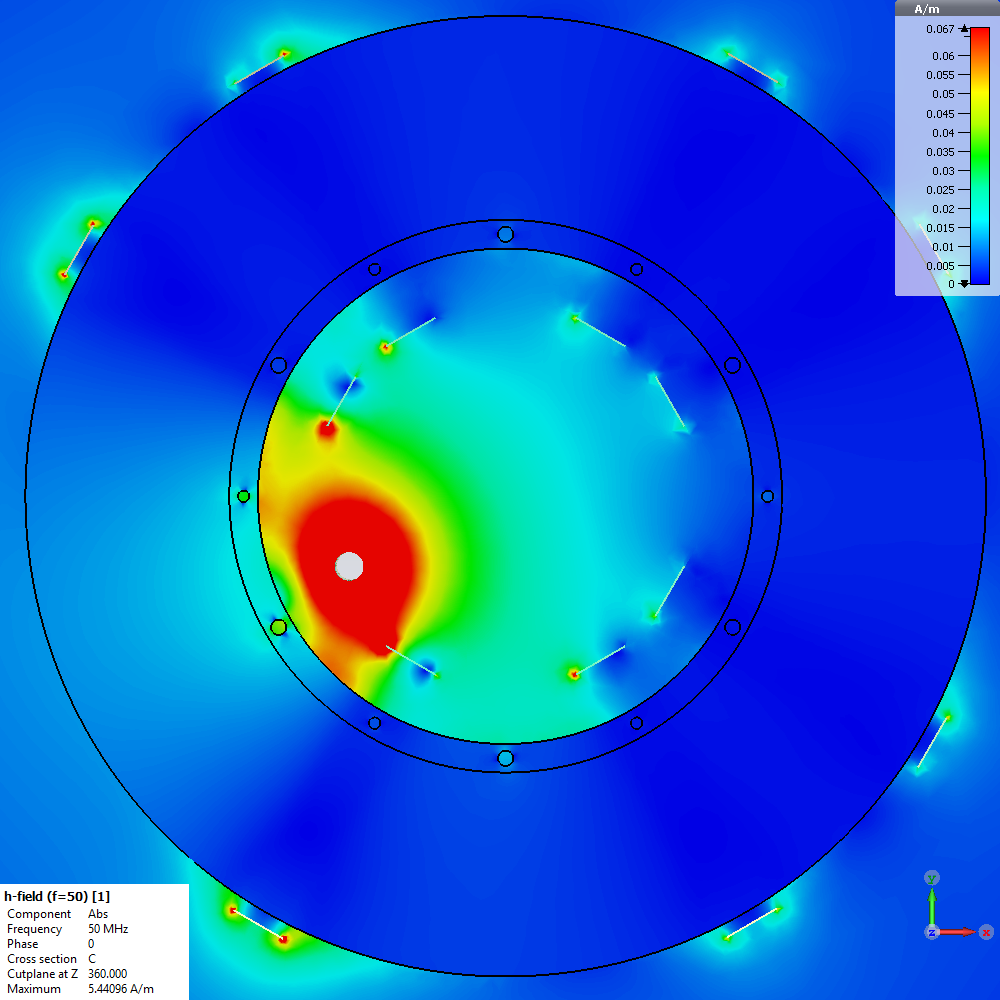
\includegraphics[width=0.33\textwidth]{Feldbilder/7KS}}
	\subfloat[8 Kurzschluss der Breite $\SI{30}{\milli\meter}$ und der h\"ohe $\SI{160}{\milli\meter}$.]{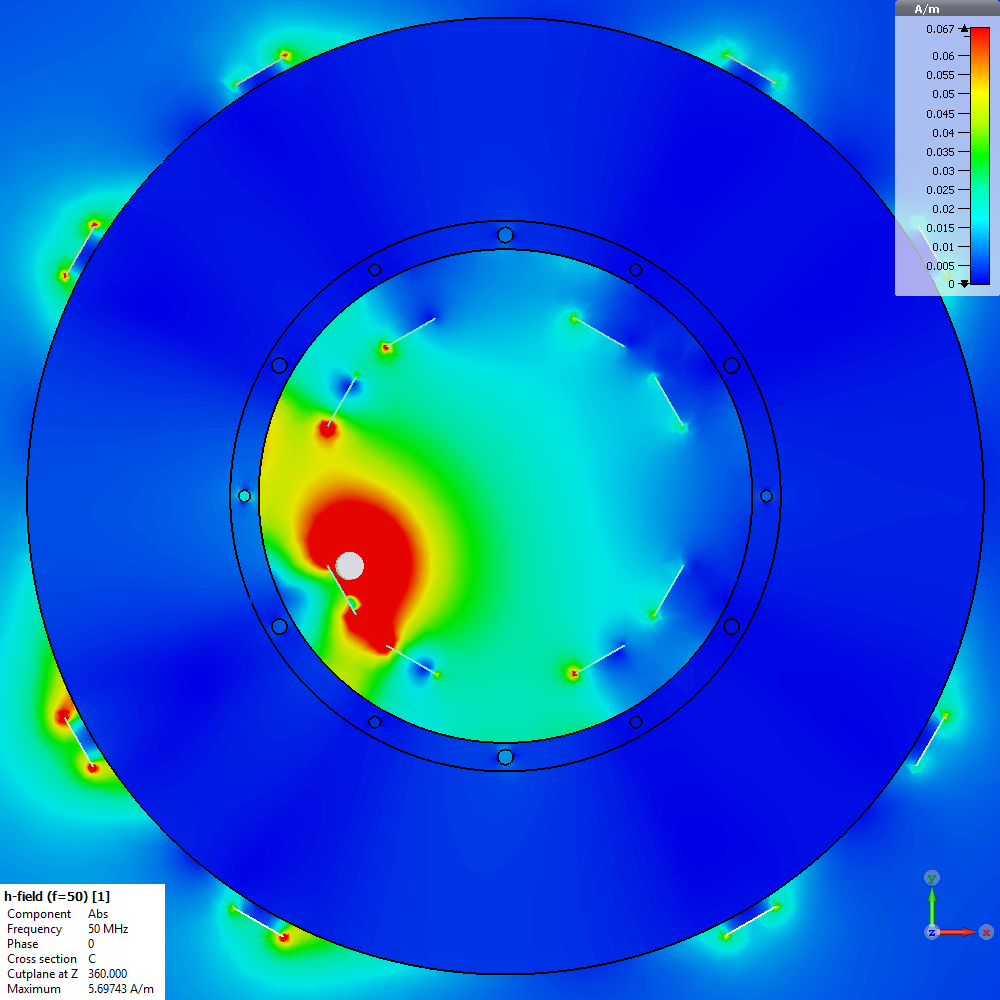
\includegraphics[width=0.33\textwidth]{Feldbilder/8KS}}
	\caption{Gegen\"uberstellung der Feldbilder des Ringkerns mit sieben und acht Kurzschl\"ussen aus der CST Simulation.}
	\label{fig:field78ks}
\end{figure}